\documentclass[tikz,border=3mm]{standalone}
\usepackage[T1]{fontenc}
\usetikzlibrary{arrows.meta,positioning}
\begin{document}
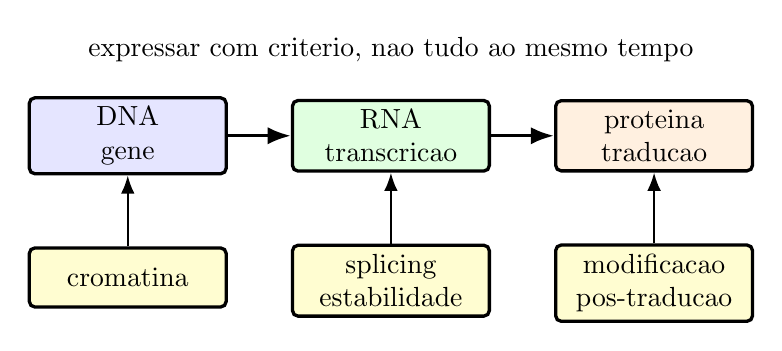
\begin{tikzpicture}[>=Latex,node distance=0.75cm]
  \tikzstyle{box}=[draw,rounded corners=2pt,very thick,align=center,minimum width=2.5cm,minimum height=0.75cm]
  \node[box,fill=blue!10] (dna) {DNA\\gene};
  \node[box,fill=green!12,right=0.8cm of dna] (rna) {RNA\\transcricao};
  \node[box,fill=orange!12,right=0.8cm of rna] (prot) {proteina\\traducao};
  \node[box,fill=yellow!18,below=0.9cm of dna] (crom) {cromatina};
  \node[box,fill=yellow!18,below=0.9cm of rna] (splice) {splicing\\estabilidade};
  \node[box,fill=yellow!18,below=0.9cm of prot] (pos) {modificacao\\pos-traducao};
  \draw[very thick,->] (dna) -- (rna);
  \draw[very thick,->] (rna) -- (prot);
  \draw[thick,->] (crom) -- (dna);
  \draw[thick,->] (splice) -- (rna);
  \draw[thick,->] (pos) -- (prot);
  \node[align=center,above=0.35cm of rna] {expressar com criterio, nao tudo ao mesmo tempo};
\end{tikzpicture}
\end{document}
